\section{Движение заряженных частиц}

\begin{ex}
Заряженная частица массы $m$ зарядом $q$ влетает в магнитное поле $B$ под углом $\alpha$ со скоростью $v$. По какой траектории движется частица? Каков пространственный период витка (шаг спирали)?
\begin{ans}
$d = 2 \pi v \cos \alpha m / qB$
\end{ans}
\end{ex}

%Ижевск
\begin{ex}
По обмотке длинного цилиндрического соленоида радиуса $R$ протекает постоянный ток, создающий внутри соленоида однородное магнитное поле с индукцией $B$. Между витками соленоида в него влетает по радиусу (перпендикулярно оси соленоида) электрон со скоростью $v$. Отклоняясь в магнитном поле, электрон спустя некоторое время покинул соленоид. Определите время движения внутри соленоида.
\begin{ans}
$t=\frac{2m}{eB}\arctan \left( \frac{eBR}{mv}\right)$
\end{ans}
\end{ex}

\begin{ex}
\hspace{0pt} \\
\begin{minipage}{.65\textwidth}
(2018) Вакуумный диод представляет собой две металлические пластины -- катод и анод. Между пластинами имеется однородное магнитное поле с индукцией $B$, параллельной плоскости пластин (направленной из плоскости чертежа). Расстояние между пластинами $d$. Из катода вылетают электроны. 1) При каких начальных скоростях все электроны не смогут достичь анода при $U = 0$? 2) При каких напряжениях $U$ все электроны не смогут достичь анода при нулевой начальной скорости?
\end{minipage}
\begin{minipage}{.35\textwidth}
\centering
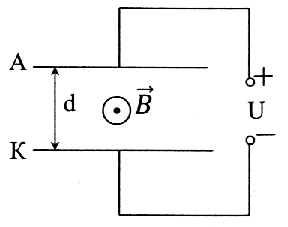
\includegraphics[width = 0.9 \textwidth]{ElectronInVacuumDiode.png}
\end{minipage}
\begin{ans}
1) $v_0 < eBd/m$; 2) $U < eB^2d^2/2m$
\end{ans}
\end{ex}

\begin{ex}
(2014) Незаряженная неподвижная частица распалась в однородном магнитном поле с индукцией $B$ на две частицы с массами $m_1$ и $m_2$ и зарядами $+q$ и $-q$. Найдите время, через которое произойдет соударение частиц. Кулоновским взаимодействием между частицами пренебречь.
\begin{ans}
$t = \frac{2\pi m_1 m_2}{qB(m_1+m_2)}$
\end{ans}
\end{ex}

\begin{ex}
(2008) Электронно-лучевая трубка помещена в однородное магнитное поле, напряженность $H$ которого перпендикулярна плоскости экрана. Электроны влетают в электронно-лучевую трубку из электронной пушки с составляющей скорости $u$ вдоль оси трубки и составляющей скорости $v_0$ перпендикулярно оси. При какой длине $L$ трубки все электроны фокусируются в одной точке экрана?
\begin{ans}
$L=2\pi m u n/ eB$, $n \in \mathcal{N}$
\end{ans}
\end{ex}

\begin{ex}
(2012) Две заряженные частицы движутся в однородном магнитном поле $B$, причем $q_1/m_1 = q_2/m_2$. Написать уравнения движения центра масс и уравнение относительного движения.
\begin{ans}
${\vec{r}_c}^{\prime \prime} = \frac{q_1}{m_1}\vec{v}_c \times \vec B$, 
${\vec{r}}^{\prime \prime} = \frac{q_1}{m_1}\vec{r}^{\prime} \times \vec B + \frac{q_1(q_2-q_1)\vec r}{m_1 r^3}$
\end{ans}
\end{ex}

\begin{ex}
(2013) Заряд $q$ движется в поле магнитного монополя $\vec{B} = \alpha \vec{r}/r^3$. Найдите интеграл движения, следующий из закона изменения момента импульса заряда.
\begin{ans}
$\vec r \times \vec p - \alpha q \vec r/ r = \text{const} $
\end{ans}
\end{ex}

\begin{ex}
Частица c зарядом $q$ и массой $m$ движется с начальной скоростью $v_0$ в вязкой среде в поперечном магнитном поле с индукцией $B$. Сила сопротивления $\vec{F} = -\gamma \vec{v}$, где $\gamma$ - константа. На каком расстоянии от начальной точки частица остановится?
\begin{sol}
На частицу действуют сила вязкого трения $\vec{F} = - r\vec{v}$ и сила Лоренца $\vec{F_L} = q \vec{v} \times \vec{B}$, уравнение движения в проекциях на оси, перпендикулярные $\vec{B}$, имеет вид:  $m \dot{v_x}=-rv_x+q v_y B$, $m \dot{v_y}=-rv_y-q v_x B$. Умножим второе из этих уравнений на $i$ и сложим с первым, получим $m\left( \dot{v_x} +i \dot{v_y} \right) = -r(v_x+i v_y) - iqB(v_x+i v_y)$. Обозначим $\phi \equiv v_x+i v_y$, тогда получим для $\phi$ дифференциальное уравнение $\dot{\phi} + \delta \phi + i\omega \phi=0$, где $\delta=r/m$,  $\omega=qB/m$. Решение этого уравнения, удовлетворяющее начальным условиям $v_x(0)=v_0$, $v_y(0)=0$, имеет вид $\phi(t)=v_0 e^{-(\delta +i\omega) t}$. Расстояние от начальной точки до точки, где частица остановится, $L=\sqrt{x_{\infty}^2 + y_{\infty}^2} =\sqrt{ \left( \int_{0}^{\infty}{v_x \, dt} \right)^2 + \left( \int_{0}^{\infty}{v_y \, dt} \right)^2}=\vert \int_{0}^{\infty}{ \phi \, dt} \vert=v_0/\sqrt{\delta^2 +\omega^2}=m v_0/\sqrt{r^2+q^2B^2}$.
\end{sol}
\begin{ans}
$r_{\infty} = mv_0/\sqrt{\gamma^2 + q^2B^2}$
\end{ans}
\end{ex}

\begin{ex}
(2007) Частица c зарядом $q$ и массой $m$ движется в постоянных однородных скрещенных полях $\vec{E} \bot \vec{H}$ в среде с малым линейным сопротивлением $\vec{F} = -\gamma \vec{v}$. Найти скорость частицы вдоль поля $\vec{E}$, усредненную по периоду.
\begin{ans}
$\langle v \rangle = \frac{E}{B}\left(\frac{\beta}{2\omega} + 2\pi \frac{\beta^2}{\omega^2} \right)$, $\beta = 2\gamma/m$, $\omega = \sqrt{\frac{q^2B^2+\gamma^2}{m^2}} \approx \frac{qB}{m}$
\end{ans}
\end{ex}

%Ижевск, Черепанов
\begin{ex}
На магнитный барьер, задаваемый в пространстве статическим магнитным полем $\vec{B} = \left(0, 0, \frac{B_0}{\cosh^2(ky)}\right)$, где $k$ -- константа, из бесконечности налетает протон с начальной скоростью $\vec{v}_{-\infty} = (0, v_0, 0)$, $\vec{r}_{-\infty} = (0, -\infty, 0)$. Оцените минимальную скорость, которую должен иметь протон, чтобы преодолеть барьер и уйти на бесконечность. 
\begin{ans}
$v_0 = 2qB_0/(mk)$
\end{ans}
\end{ex}

%Черепанов
\begin{ex}
(2005)  Магнетрон -- это прибор, состоящий из нити накала радиуса $a$ и коаксиального цилиндрического анода радиуса $b$, которые находятся в однородном магнитном поле параллельном нити. Между нитью и анодом приложена ускоряющая разность потенциалов $U$. Найти минимальное значение индукции магнитного поля $B$, при котором электроны, вылетающие с нулевой начальной скоростью из нити, не будут достигать анода.
\begin{ans}
$B=\frac{b}{b^2-a^2}\sqrt{\frac{8mU}{e}}$
\end{ans}
\end{ex}